%% ============================================================
%%  Reddit-Augmented Reinforcement Learning for Stock Trading
%%  CS 5180 Final Project -- Spring 2026
%%  AAAI-style two-column layout (aaai2026.sty approximated)
%% ============================================================
\documentclass[letterpaper,twocolumn]{article}

\usepackage{times}
\usepackage{helvet}
\usepackage{courier}
\usepackage[T1]{fontenc}
\usepackage[utf8]{inputenc}
\usepackage{amsmath,amssymb}
\usepackage{graphicx}
\usepackage{booktabs}
\usepackage{xcolor}
\usepackage[hyphens]{url}
\usepackage{natbib}
\usepackage{array}
\usepackage{geometry}
\frenchspacing

\geometry{
  letterpaper,
  top=1.0in, bottom=1.0in,
  left=0.75in, right=0.75in,
  columnsep=0.25in
}

\graphicspath{{results/figures/}{results/plots/}}

% ─────────────────────────────────────────────────────────────
\begin{document}

\title{\textbf{Can Reddit Make a Better Stock Trader?\\
Deep Reinforcement Learning with Social Media\\
Embeddings on Meme Stocks}}

\author{
  Ananya Parag Joshi \\
  {\small Khoury College of Computer Sciences} \\
  {\small Northeastern University, Boston, MA} \\
  {\small \texttt{joshi.an@northeastern.edu}}
}
\date{}
\maketitle

% ─────────────────────────────────────────────────────────────
\begin{abstract}
This paper trains deep reinforcement learning agents to trade
four stocks (GME, TSLA, AAPL, and AMC) and asks whether
adding Reddit post embeddings to the agent's observations
actually improves performance.
Two algorithms, Proximal Policy Optimization (PPO) and
Deep Q-Networks (DQN), are each run with and without
384-dimensional Sentence-BERT encodings of daily Reddit
activity.
On the main test set, adding Reddit helps clearly for TSLA
(DQN Sharpe 1.693 vs 1.215 for buy-and-hold) and
meaningfully for AAPL, while all agents correctly sit out
AMC's 57\% decline.
GME is the interesting outlier: Reddit should matter most
there, but walk-forward validation over 2022--2024 shows
that the Reddit signal actually hurts the agent on GME in
post-squeeze years, because the community stayed bullish
long after the stock stopped responding to sentiment.
Walk-forward results over 2022--2024 show that Reddit helps
most on stocks where community sentiment leads price (TSLA,
AMC in volatile regimes) and provides little marginal benefit
on institutionally driven stocks like AAPL, which all models
trade profitably regardless of whether Reddit is included.
\end{abstract}

% ─────────────────────────────────────────────────────────────
\section{Introduction}

In January 2021 a coordinated group of retail investors on
r/WallStreetBets drove GameStop's stock up over 1,700\%
in two weeks \citep{reddit2021gamestop}.
The event was unusual enough to trigger congressional hearings,
but it also raised a genuine research question: if Reddit was
causing price moves that large, should a trading agent be
reading Reddit?

Most quantitative trading systems ignore social media entirely
and rely on price history and technical indicators.
Reinforcement learning (RL) offers a convenient way to test
whether social media adds anything, because the agent can be
given observations with and without Reddit features and the
two variants can be directly compared.
An RL agent treats trading as a sequential decision problem:
every day it sees the current market state, picks an action
(buy, hold, or sell), and receives a reward based on whether
the portfolio value went up or down \citep{moody1998performance}.
Deep RL scales this to high-dimensional inputs by using a
neural network to represent the policy or value function
\citep{mnih2015human,schulman2017proximal}.

The four stocks chosen here cover different relationships with
Reddit.
GME and AMC are the original meme stocks, where Reddit was
arguably the primary driver of price in 2021.
TSLA has an enormous and active community on r/wallstreetbets
and r/investing.
AAPL is included as a control. It is one of the most widely
held stocks and its price is driven more by earnings and
macro factors than by retail sentiment.
If Reddit embeddings help more on GME/TSLA/AMC than on AAPL,
that is evidence that the signal is genuine rather than noise.

The main question this paper tries to answer is: \textit{when
does Reddit actually help a trading agent, and when does it
not?}

% ─────────────────────────────────────────────────────────────
\section{Background}

\subsection{Reinforcement Learning for Trading}

A trading agent can be modeled as a Markov Decision Process
(MDP) $\langle \mathcal{S}, \mathcal{A}, \mathcal{P},
\mathcal{R}, \gamma \rangle$ where $\mathcal{S}$ is the set
of market states, $\mathcal{A}$ is the set of actions, and
$\mathcal{R}$ is the reward signal \citep{sutton2018reinforcement}.
At each trading day $t$ the agent observes $s_t$, selects an
action $a_t \in \{\text{hold, buy, sell}\}$, and receives a
reward $r_t$ reflecting the change in portfolio value.
The objective is to find a policy $\pi: \mathcal{S} \to
\mathcal{A}$ that maximises expected cumulative discounted
reward $\mathbb{E}[\sum_{t} \gamma^t r_t]$.

\subsection{Proximal Policy Optimization}

PPO \citep{schulman2017proximal} is an actor-critic algorithm
that keeps policy updates conservative by clipping the
importance-sampling ratio:
\begin{equation}
  \mathcal{L}^{\text{clip}}(\theta) =
    \mathbb{E}_t\!\Bigl[
      \min\bigl(
        r_t(\theta)\hat{A}_t,\;
        \mathrm{clip}(r_t(\theta),\, 1\!-\!\varepsilon,\,
                     1\!+\!\varepsilon)\hat{A}_t
      \bigr)
    \Bigr],
\end{equation}
where $r_t(\theta) = \pi_\theta(a_t\mid s_t) /
\pi_{\theta_\text{old}}(a_t\mid s_t)$ and $\hat{A}_t$ is
the generalized advantage estimate \citep{schulman2015high}.
The clipping prevents a single bad update from collapsing the
policy, which matters in a noisy financial environment.

\subsection{Deep Q-Networks}

DQN \citep{mnih2015human} learns an action-value function
$Q(s,a;\theta)$ by minimising the temporal difference error:
\begin{equation}
  \mathcal{L}(\theta) = \mathbb{E}\!\Bigl[
    \bigl(r + \gamma \max_{a'} Q(s',a';\theta^{-})
    - Q(s,a;\theta)\bigr)^2
  \Bigr],
\end{equation}
where $\theta^{-}$ are the target network weights, updated
every 1000 steps.
DQN is off-policy and uses experience replay, which means it
can revisit rare high-reward events repeatedly during training.
This turns out to matter for trading: significant sentiment
spikes happen infrequently, and being able to reuse those
experiences helps the agent learn their value.

\subsection{Sentence-BERT Embeddings}

Sentence-BERT \citep{reimers2019sentence} fine-tunes a BERT
encoder \citep{devlin2019bert} with a siamese network
objective so that semantically similar sentences are mapped
to nearby points in a fixed-size vector space.
Common pre-trained variants such as \texttt{all-MiniLM-L6-v2}
produce 384-dimensional dense embeddings from short text inputs.
The advantage over simpler polarity scores or bag-of-words
counts is that the embedding preserves semantic content:
``the shorts are getting squeezed'' and ``the stock is
recovering from a squeeze'' produce different vectors even
though they share many keywords, and that distinction carries
real information for a trading agent reading Reddit posts.

% ─────────────────────────────────────────────────────────────
\section{Related Work}

Twitter mood was shown to predict DJIA movements up to four
days ahead \citep{bollen2011twitter}, and topic-based Twitter
sentiment can improve individual stock price predictions
\citep{si2013exploiting}.
These approaches produce a prediction but do not learn a
trading policy.

On the RL side, \citet{deng2016deep} used recurrent networks
with RL for trading signals.
\citet{jiang2017deep} framed portfolio management as an RL
problem.
\citet{yang2020deep} combined PPO, A2C, and DDPG in an
ensemble strategy for multi-stock trading.
\citet{liu2020adaptive} added technical indicators as
additional state features for an adaptive RL trader.
None of these incorporate Reddit or any social media signal
specifically tied to meme stocks.

The closest work to this paper combines NLP sentiment with RL for
trading \citep{si2013exploiting}, but uses coarse bag-of-words
features rather than dense embeddings, and does not study the
regime-dependence of the signal (i.e., when it helps and
when it does not).

% ─────────────────────────────────────────────────────────────
\section{Methods}

\subsection{Environment}

The trading environment is built with Gymnasium
\citep{gymnasium}.
The agent controls a single-asset account starting with
\$10,000.
On each trading day it selects one of three actions:
hold (0), buy all (1), or sell all (2).

\smallskip
\noindent\textbf{Observation space.}
With Reddit enabled, the observation on day $t$ is:
\begin{equation}
  s_t = \bigl[
    \underbrace{r_t,\, z^V_t,\, \sigma_t,\, \rho_t,\,
    \mu_t}_{\text{5 price features}},\;
    \underbrace{p_t,\, q_t,\, c_t}_{\text{3 Reddit scalars}},\;
    \underbrace{\mathbf{e}_t}_{\in\mathbb{R}^{384}}
  \bigr] \in \mathbb{R}^{392}.
\end{equation}
Without Reddit the observation is just the 5 price features.

\smallskip
\noindent\textbf{Market features.}
Each of the five price features is computed daily from
closing price $P_t$ and volume $V_t$:

\noindent\textit{Daily return.}
Simple percentage change in closing price:
\begin{equation}
  r_t = \frac{P_t - P_{t-1}}{P_{t-1}}.
\end{equation}

\noindent\textit{Volume z-score.}
How unusual today's volume is relative to the past 20 days:
\begin{equation}
  z^V_t = \frac{V_t - \overline{V}_{20,t}}{\hat{\sigma}^V_{20,t}},
\end{equation}
where $\overline{V}_{20,t}$ and $\hat{\sigma}^V_{20,t}$ are
the 20-day rolling mean and standard deviation of volume.
A large positive value means unusually high trading activity.

\noindent\textit{Volatility.}
Five-day rolling standard deviation of daily returns,
capturing how erratic price has been recently:
\begin{equation}
  \sigma_t = \sqrt{\frac{1}{4}\sum_{k=0}^{4}(r_{t-k} - \bar{r})^2}.
\end{equation}
This also appears as the volatility penalty in the reward
function.

\noindent\textit{Relative Strength Index (RSI).}
A momentum indicator over a 14-day window.
Let $U_t = \max(r_t,0)$ be the day's gain and
$D_t = \max(-r_t,0)$ its loss.
The average gain and loss over $n=14$ days are:
\begin{equation}
  \overline{U}_t = \tfrac{1}{n}\textstyle\sum_{k=0}^{n-1}U_{t-k},
  \quad
  \overline{D}_t = \tfrac{1}{n}\textstyle\sum_{k=0}^{n-1}D_{t-k}.
\end{equation}
Then:
\begin{equation}
  \text{RSI}_t = 100 - \frac{100}{1 + \overline{U}_t/\overline{D}_t},
  \qquad
  \rho_t = \frac{\text{RSI}_t}{100} \in [0,1].
\end{equation}
Values near 1 indicate a stock is overbought; near 0, oversold.

\noindent\textit{Moving average crossover.}
A binary signal indicating whether the 10-day simple moving
average is above the 50-day:
\begin{equation}
  \mu_t = \mathbf{1}\!\left[
    \text{SMA}_{10}(P)_t > \text{SMA}_{50}(P)_t
  \right] \in \{0,1\}.
\end{equation}
When $\mu_t = 1$ the short-term trend is above the long-term
trend, which is a conventional buy signal in technical
analysis.

\smallskip
\noindent\textbf{Reddit scalar features.}
$p_t$, $q_t$, $c_t$ are the post count, average upvote score,
and average comment count for the ticker on day $t$, each
normalised to $[0,1]$ by the per-ticker maximum seen during
training.
$\mathbf{e}_t \in \mathbb{R}^{384}$ is the mean of the
Sentence-BERT embeddings of all individual post titles for
that day.
On days with no Reddit activity, all Reddit features are
set to zero.

\smallskip
\noindent\textbf{Reward function.}
\begin{equation}
  r(s_t, a_t) = \frac{\Delta V_t}{V_t}
    - 0.1\,\sigma_t
    - 0.001\cdot\mathbf{1}[\text{trade}],
\end{equation}
The first term is the daily portfolio return.
The volatility term penalises holding during highly volatile
periods to encourage the agent to manage downside risk.
The trade cost of 0.1\% is applied each time a buy or sell
is executed.

\subsection{Data}

\textbf{Price data.}
Daily OHLCV data for GME, TSLA, AAPL, and AMC covering
2019 through 2024.
Technical features are computed from close prices and
aligned to trading days.

\noindent\textbf{Reddit data.}
Posts scraped from r/WallStreetBets, r/stocks, r/investing,
and ticker-specific subreddits.
Post titles for each ticker are grouped by day; each title is
encoded separately with \texttt{all-MiniLM-L6-v2} and the
resulting 384-dimensional vectors are mean-pooled to produce
one daily embedding per ticker.
On days with no activity the embedding is zero.
The scalar features (post count, score, comments) are
normalised to $[0,1]$ by their per-ticker maximum over the
training window.

\noindent\textbf{Train/test splits.}
The \emph{fixed 80/20 split} divides the full 2019--2024
dataset chronologically: the first 80\% of trading days
(through October~23, 2023) are used for training and the
remaining 20\% (October~24, 2023 through December~30, 2024)
for testing.
The \emph{walk-forward evaluation} tests three separate
one-year windows: 2022, 2023, and 2024, each time training
on all data available before that year.

\subsection{Training}

PPO and DQN are implemented with Stable-Baselines3
\citep{stable_baselines3} using a two-layer MLP policy
(64 units each).
Both algorithms train for 500,000 timesteps.
PPO uses learning rate $3\times10^{-4}$, $n_\text{steps}=256$,
clip range 0.2, $\gamma=0.99$, and GAE $\lambda=0.95$.
DQN uses learning rate $10^{-4}$, replay buffer of 50,000
transitions, and $\varepsilon$-greedy exploration decaying
from 1.0 to 0.05 over the first 30\% of training.
A separate model is trained for each ticker--algorithm
combination, giving 12 models total (3 algorithms $\times$
4 tickers).

\subsection{Metrics}

Three metrics are reported throughout.

\noindent\textit{Cumulative return} measures raw profitability
over the test period of $T$ trading days:
\begin{equation}
  \text{Return} = \frac{V_T - V_0}{V_0},
\end{equation}
where $V_0 = \$10{,}000$ and $V_T$ is the final portfolio value.

\noindent\textit{Sharpe ratio} \citep{sharpe1994sharpe} adjusts
return for the risk taken. Using daily portfolio returns
$\{r^p_t\}$ with mean $\bar{r}^p$ and standard deviation
$\sigma^p$:
\begin{equation}
  \text{Sharpe} = \frac{\bar{r}^p \cdot \sqrt{252}}{\sigma^p}.
\end{equation}
The $\sqrt{252}$ factor annualises the ratio (252 trading days
per year). Values above 1.0 are generally considered
acceptable; above 2.0 is strong.

\noindent\textit{Maximum drawdown} records the worst
peak-to-trough portfolio loss over the test period:
\begin{equation}
  \text{MDD} = \min_{t} \frac{V_t - \max_{s \leq t} V_s}{\max_{s \leq t} V_s}.
\end{equation}
A value of $-0.25$ means the portfolio fell 25\% from its
highest point at some moment during the test period.

% ─────────────────────────────────────────────────────────────
\section{Experiments and Results}

\subsection{80/20 Test Results}

Table~\ref{tab:main} shows all models on the fixed 80/20 test
split, and Figures~\ref{fig:returns}--\ref{fig:drawdown}
visualise cumulative return, Sharpe ratio, and maximum
drawdown.

\begin{table*}[t]
\centering
\caption{80/20 test-set results. Initial portfolio value
\$10{,}000 for all agents.
Bold indicates the best value per metric and ticker
(excluding drawdown for AMC since all RL agents have 0\%).}
\label{tab:main}
\setlength{\tabcolsep}{4.5pt}
\begin{tabular}{llrrrrr}
\toprule
\textbf{Ticker} & \textbf{Model} &
\textbf{Final (\$)} & \textbf{Return (\%)} &
\textbf{Sharpe} & \textbf{Max DD (\%)} & \textbf{Trades} \\
\midrule
GME & PPO + Reddit    & 23{,}687 & \textbf{136.87} & 1.145 & $-62.42$ & 1  \\
    & PPO no Reddit   & 22{,}210 & 122.10           & 1.075 & $-18.95$ & 12 \\
    & DQN + Reddit    & 23{,}687 & \textbf{136.87} & 1.145 & $-62.42$ & 1  \\
    & Buy-and-Hold    & 22{,}795 & 127.95           & 1.120 & $-62.41$ & 1  \\
\midrule
TSLA & PPO + Reddit   & 21{,}713 & 117.13           & 1.453 & $-29.88$ & 1  \\
     & PPO no Reddit  & 19{,}231 & 92.31            & 1.245 & $-45.55$ & 1  \\
     & DQN + Reddit   & \textbf{22{,}811} & \textbf{128.11} & \textbf{1.693} & \textbf{$-24.95$} & 35 \\
     & Buy-and-Hold   & 19{,}241 & 92.41            & 1.215 & $-45.51$ & 1  \\
\midrule
AAPL & PPO + Reddit   & \textbf{15{,}142} & \textbf{51.42} & \textbf{1.750} & $-16.48$ & 1  \\
     & PPO no Reddit  & 14{,}811 & 48.11            & 1.643 & $-16.59$ & 1  \\
     & DQN + Reddit   & 14{,}838 & 48.38            & 1.746 & \textbf{$-11.69$} & 23 \\
     & Buy-and-Hold   & 14{,}605 & 46.05            & 1.589 & $-16.52$ & 1  \\
\midrule
AMC  & PPO + Reddit   & 10{,}000 & 0.00             & 0.000 & 0.00     & 0  \\
     & PPO no Reddit  & 10{,}000 & 0.00             & 0.000 & 0.00     & 0  \\
     & DQN + Reddit   & 10{,}000 & 0.00             & 0.000 & 0.00     & 0  \\
     & Buy-and-Hold   & 4{,}259  & $-57.41$         & $-0.22$ & $-77.39$ & 1 \\
\bottomrule
\end{tabular}
\end{table*}

\begin{figure}[t]
  \centering
  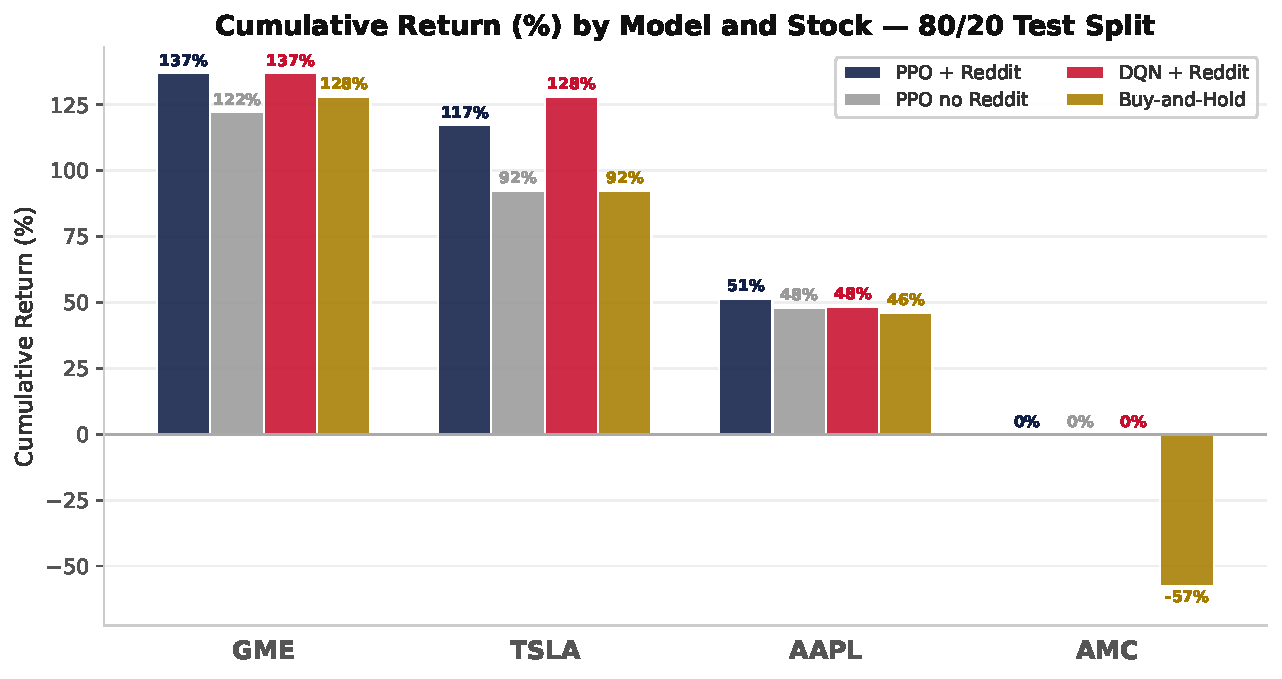
\includegraphics[width=\columnwidth]{return_comparison.pdf}
  \caption{Cumulative return (\%) on the 80/20 test split.
           All three RL agents end flat on AMC rather than
           losing 57\%. DQN + Reddit wins on TSLA;
           both Reddit agents tie for the top on GME.}
  \label{fig:returns}
\end{figure}

\begin{figure}[t]
  \centering
  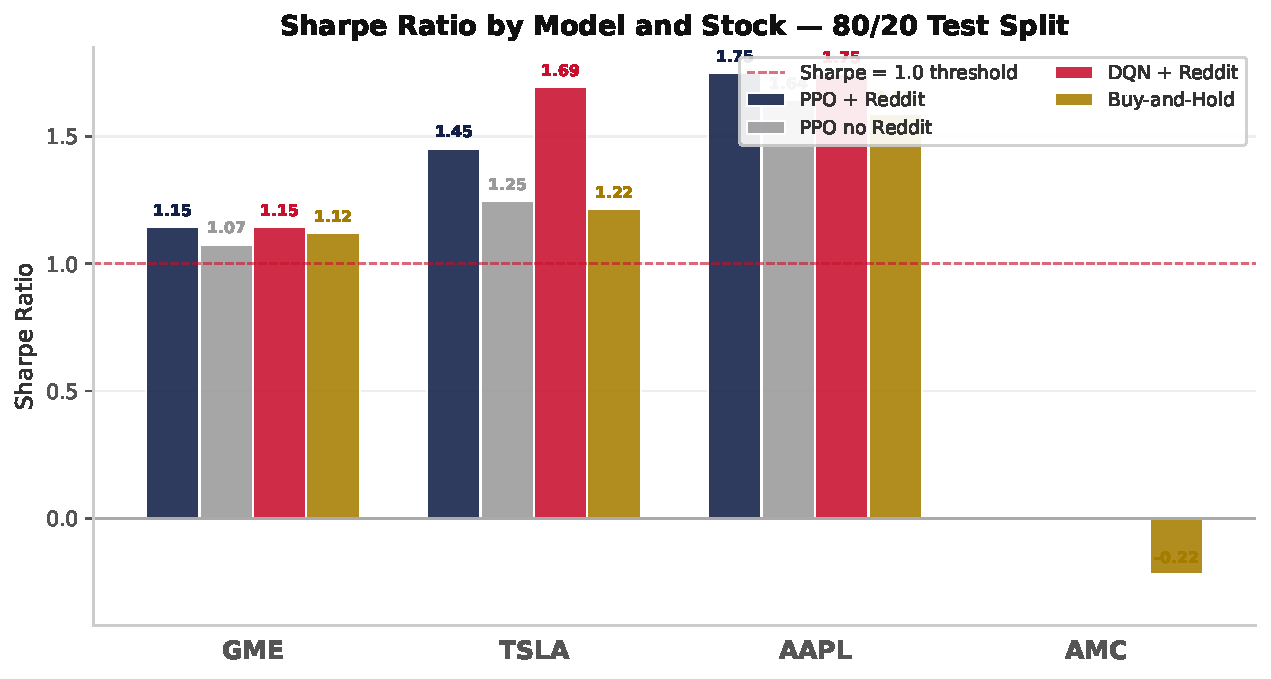
\includegraphics[width=\columnwidth]{sharpe_comparison.pdf}
  \caption{Sharpe ratio on the 80/20 test split.
           Dashed line marks Sharpe $= 1.0$.
           DQN + Reddit achieves 1.693 on TSLA, the highest
           risk-adjusted return across all ticker-model pairs.}
  \label{fig:sharpe}
\end{figure}

\begin{figure}[t]
  \centering
  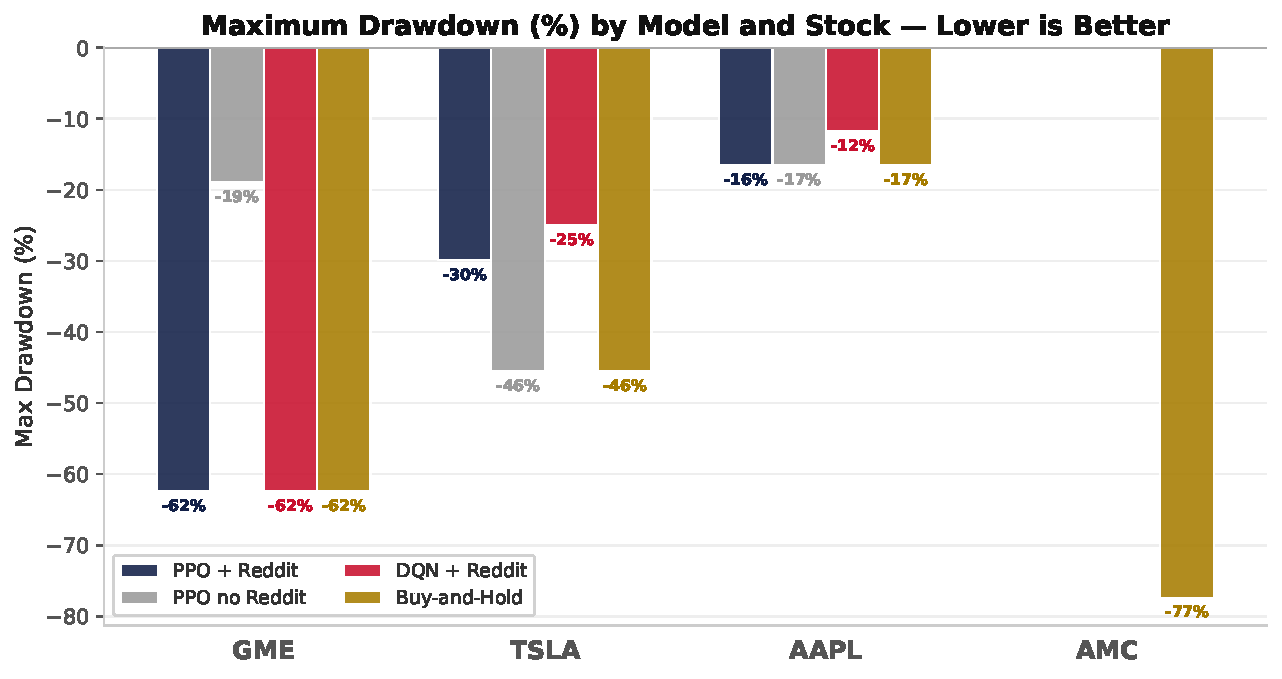
\includegraphics[width=\columnwidth]{drawdown_comparison.pdf}
  \caption{Max drawdown (\%) on the 80/20 test split.
           Lower magnitude is better. DQN + Reddit cuts
           TSLA's drawdown nearly in half compared to
           buy-and-hold ($-24.95\%$ vs $-45.51\%$).}
  \label{fig:drawdown}
\end{figure}

\textbf{TSLA.} Reddit makes the biggest difference here.
DQN with Reddit achieves a 128\% return and Sharpe of 1.693,
compared to buy-and-hold at 92\% and Sharpe 1.215.
What is striking is the drawdown reduction: DQN sells out of
positions during bad stretches (35 trades over the test
period), cutting maximum drawdown from $-45\%$ to $-25\%$.
PPO with Reddit also outperforms its no-Reddit counterpart
(117\% vs 92\% return, Sharpe 1.453 vs 1.245), confirming
the result holds across both algorithms.
TSLA is heavily discussed on Reddit and the community's
reaction to Elon Musk's activity has moved the stock
historically, which likely explains why the embedding carries
real signal here.

\textbf{AAPL.} The improvement from Reddit is small but consistent.
PPO with Reddit reaches a Sharpe of 1.750 vs 1.589 for
buy-and-hold, and DQN with Reddit holds the lowest drawdown
at $-11.69\%$.
The gains are modest compared to TSLA, which is expected.
AAPL's price is driven mainly by earnings, product launches,
and broader market conditions, not by what Reddit thinks.
The Reddit embedding still adds something, possibly encoding
general market sentiment rather than AAPL-specific
information, but it is not the dominant signal.

\textbf{AMC.} Staying out was the right call.
Every RL agent ends the test period with exactly \$10,000 and
zero trades, while buy-and-hold loses 57\% of the initial
investment.
AMC's stock was in a sustained decline over the test period
as the original meme-stock enthusiasm from 2021 faded.
The agents learned to sit on cash rather than participate,
which is the correct decision in hindsight.
Whether Reddit helped the agents identify this (by encoding
declining community engagement) or whether the price features
alone were sufficient is harder to separate.
The ablation shows no difference between with-Reddit and
no-Reddit PPO on AMC in this split, suggesting the price
signal was enough to stay out.

\textbf{GME.} This is the complicated case.
Both PPO and DQN with Reddit achieve 136.87\% return, beating
buy-and-hold (127.95\%) and PPO without Reddit (122.10\%).
On the surface this looks like a win for Reddit.
The story becomes more complicated in walk-forward validation
(Section~\ref{sec:wf}), which is where the real lesson for
GME lives.
The 80/20 test period here covers approximately 2023--2024,
which includes GME's May 2024 spike driven by Roaring Kitty's
return to social media.
In that specific window Reddit \emph{was} predictive again,
explaining the good result.
But this was a narrow window.

\subsection{Ablation: Reddit vs.\ No-Reddit}

Figure~\ref{fig:ablation} shows a direct comparison of
PPO with and without Reddit across all four tickers.

\begin{figure}[t]
  \centering
  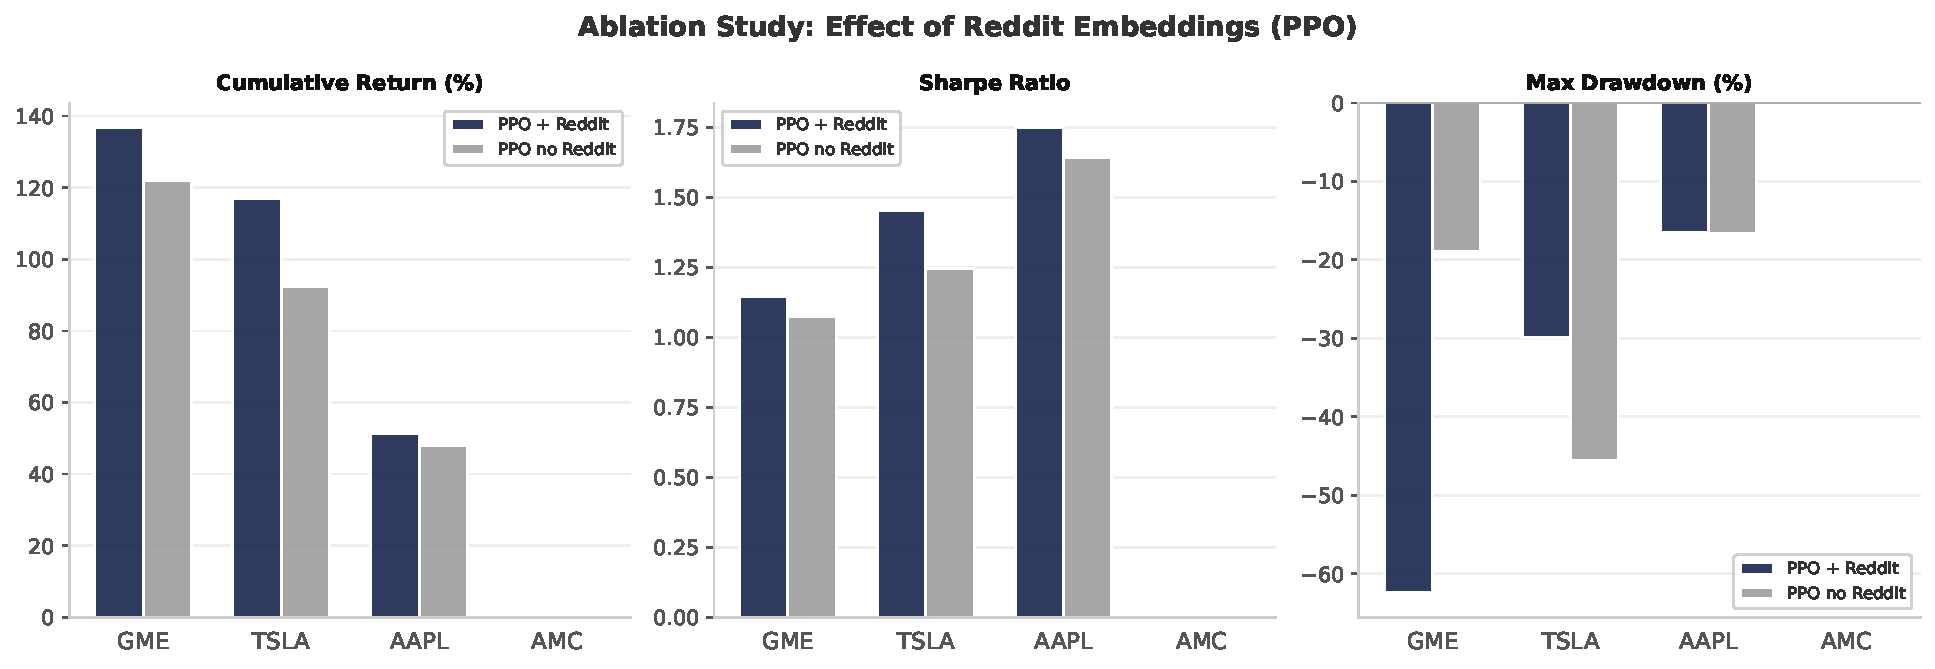
\includegraphics[width=\columnwidth]{ablation_study.pdf}
  \caption{PPO with Reddit vs.\ PPO without Reddit.
           Reddit adds the most on TSLA (+24.8 pp in return,
           +0.21 Sharpe). On AAPL the gain is smaller.
           On GME and AMC the difference is negligible in this
           split.}
  \label{fig:ablation}
\end{figure}

The results are consistent: Reddit improves TSLA clearly,
improves AAPL modestly, and makes essentially no difference
on GME and AMC in the 80/20 split.
The lack of a Reddit effect on AMC is not surprising given
that both agents hit on the same strategy (hold cash).
The lack of an effect on GME here is misleading, as the
walk-forward results make clear.

\subsection{Training Curves}
\label{sec:training}

Figure~\ref{fig:learning} shows mean evaluation reward per
episode during training, smoothed with a 9-point rolling
mean, for PPO + Reddit, PPO no Reddit, and DQN + Reddit on
each ticker.

\begin{figure}[t]
  \centering
  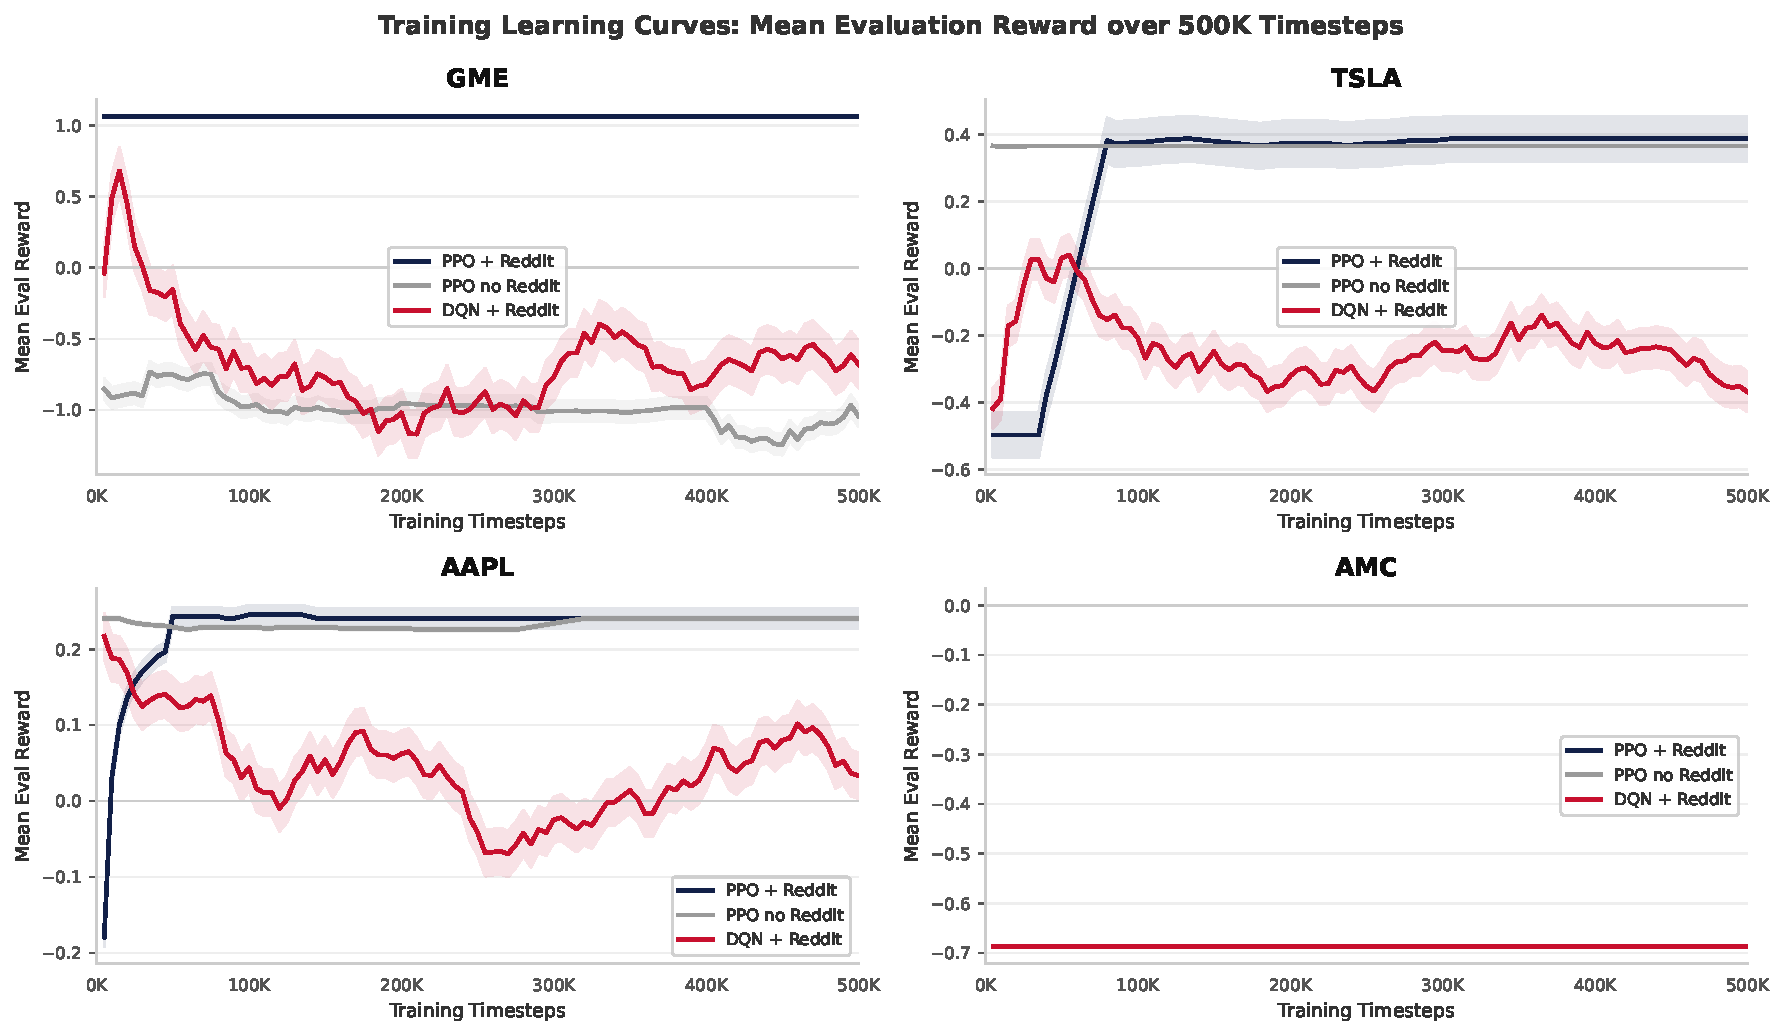
\includegraphics[width=\columnwidth]{learning_curves.pdf}
  \caption{Mean episode reward (9-point rolling average)
           over 500{,}000 training timesteps for each ticker.
           Shaded bands show $\pm 1$ standard deviation
           across evaluation checkpoints.
           All agents converge before step 200{,}000.
           Reddit agents show higher early variance on GME
           and TSLA due to the larger 392-dimensional
           observation space.}
  \label{fig:learning}
\end{figure}

All agents converge within the first 200{,}000 timesteps.
On TSLA and AAPL, PPO + Reddit consistently reaches higher
final reward than PPO without Reddit, consistent with the
test results.
On GME, training rewards are similar across all variants.
This mirrors the 80/20 results where the Reddit signal adds
only marginal benefit on GME in the main split: the agent
does not confidently exploit the Reddit embedding during
training, so the gap at test time is also small.
DQN + Reddit shows faster early improvement on TSLA, which
corresponds to its strong final test performance on that
ticker.
On AMC, all agents converge within the first 20{,}000 steps,
but to qualitatively different policies: PPO + Reddit settles
to a flat reward near zero (the hold-cash policy) while DQN
converges to a consistently loss-making trajectory, reflecting
the difference in how an on-policy actor-critic versus an
off-policy Q-learner handles a stock in sustained decline
during the training period.

\subsection{Walk-Forward Validation}
\label{sec:wf}

Rather than relying on a single train/test split, the
walk-forward evaluation tests each year separately after
training on all data up to that point.
This better reflects what a real trading system faces: the
model only knows what has happened so far and must adapt to
new market conditions each year.
The three test years cover meaningfully different regimes:
2022 was a steep bear market (the Fed raised rates aggressively
and tech stocks fell hard), 2023 was a recovery with a strong
bull run in the second half, and 2024 was mixed.

Figures~\ref{fig:wf_sharpe} and \ref{fig:wf_return} show
results by year.
Table~\ref{tab:wf_summary} summarises mean and standard
deviation of Sharpe across all three windows.
Figure~\ref{fig:wf_summary} visualises the summary.

\begin{figure*}[t]
  \centering
  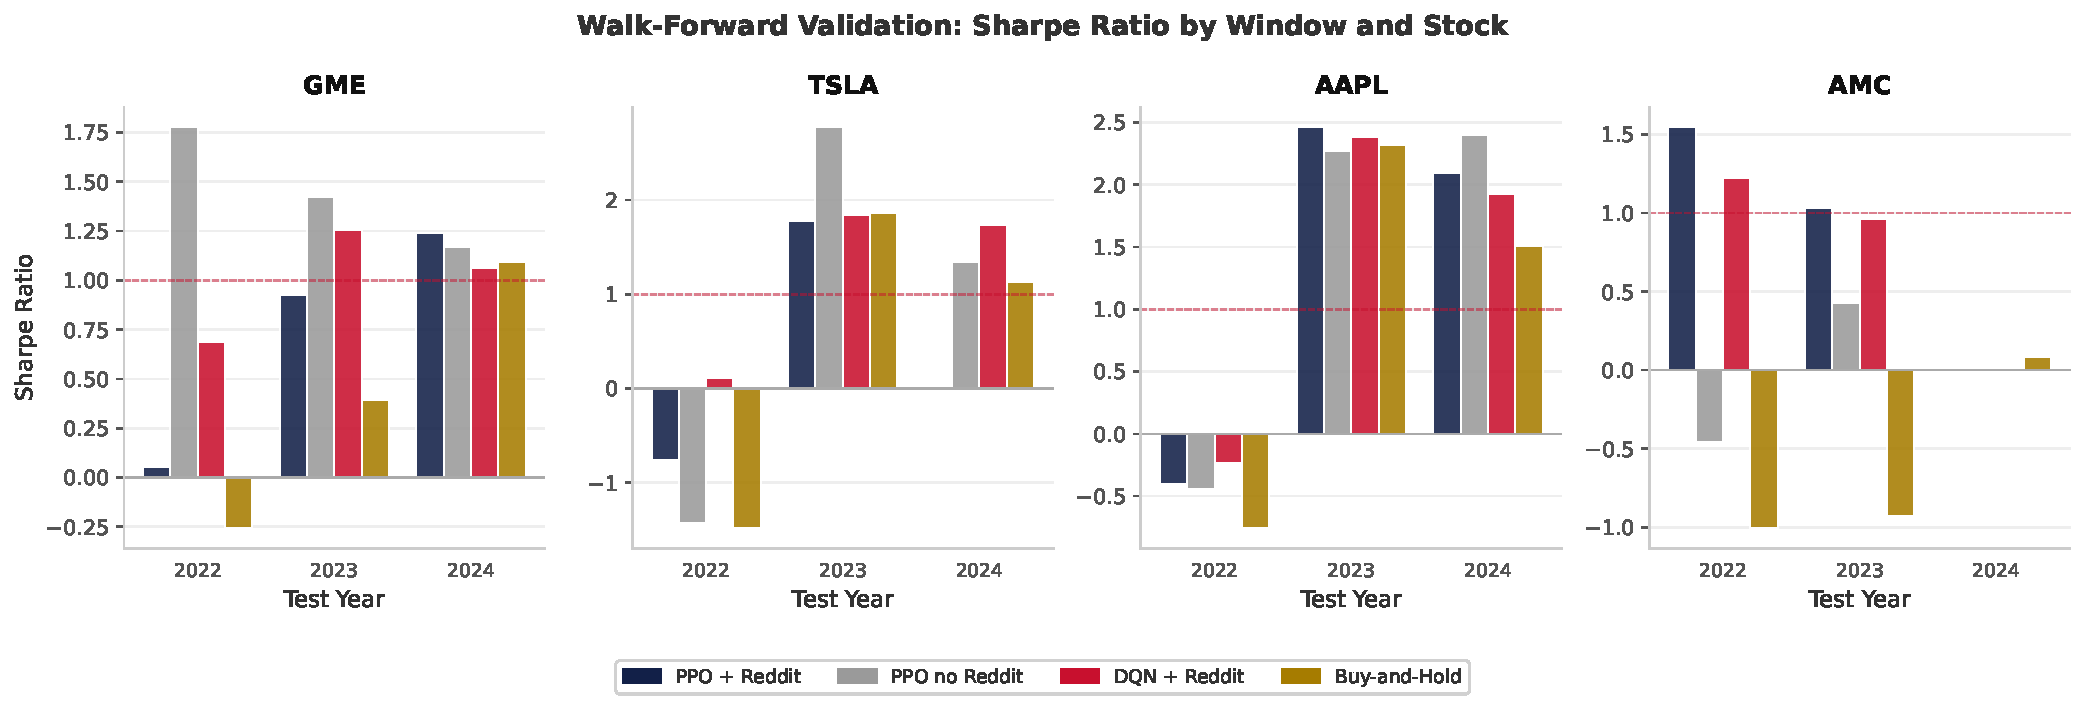
\includegraphics[width=\textwidth]{walk_forward_sharpe.pdf}
  \caption{Walk-forward Sharpe ratios by test year and ticker.
           Dashed line at Sharpe $= 1.0$.
           2022 is where the Reddit signal helps most on AMC.
           On GME in 2022--2023, PPO no Reddit consistently
           outperforms PPO + Reddit.}
  \label{fig:wf_sharpe}
\end{figure*}

\begin{figure*}[t]
  \centering
  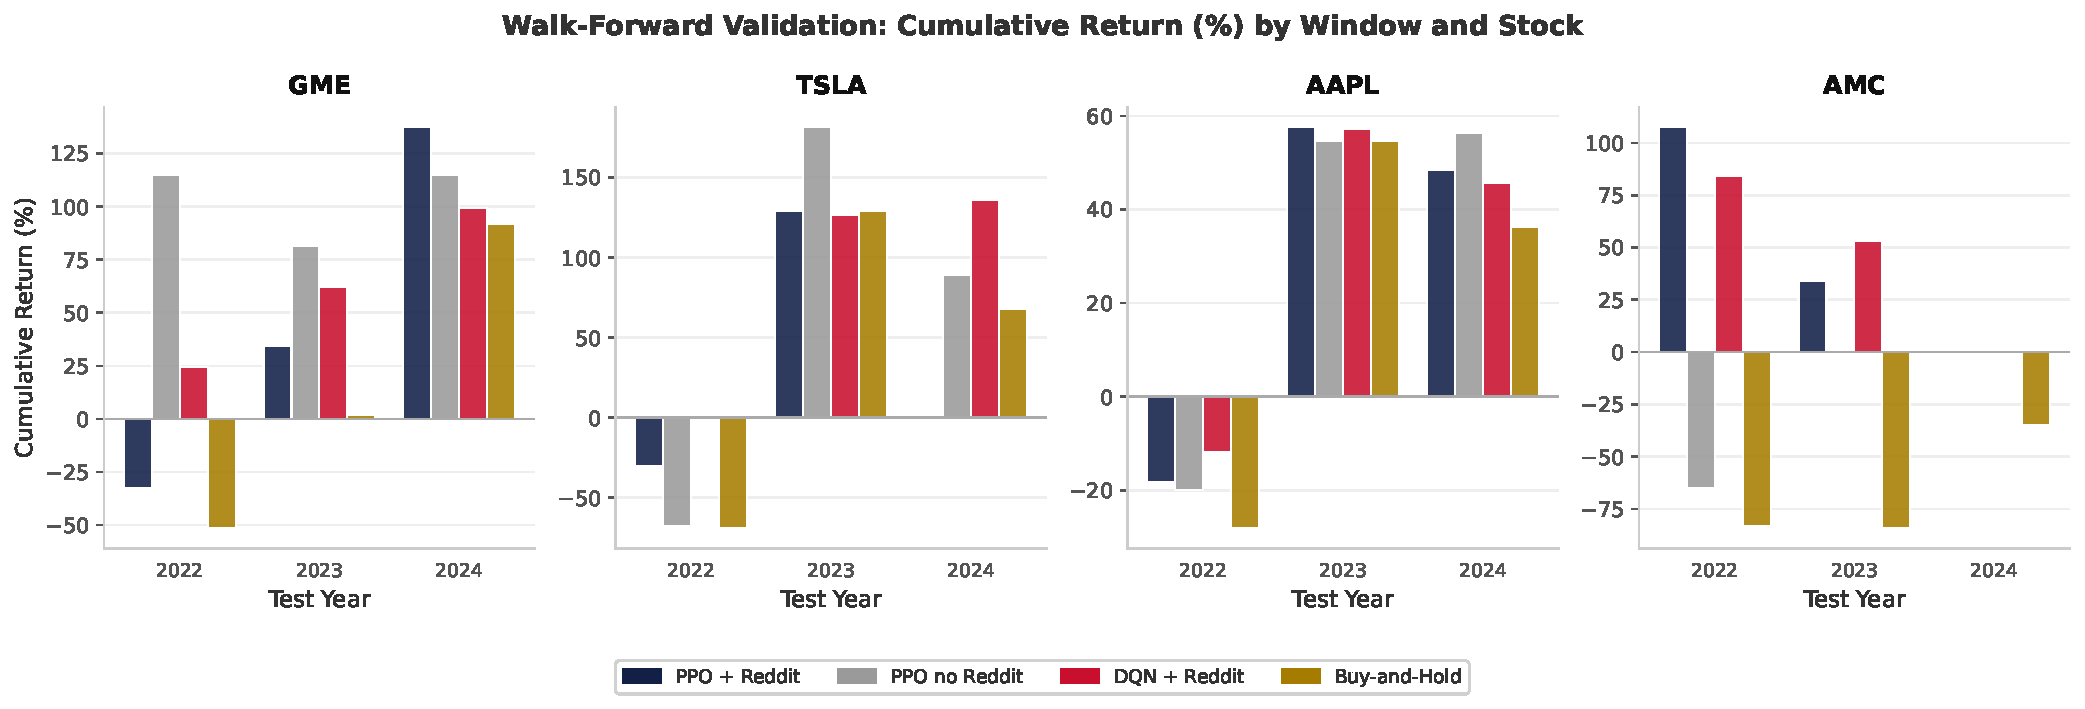
\includegraphics[width=\textwidth]{walk_forward_return.pdf}
  \caption{Walk-forward cumulative returns by year.
           The most striking result is AMC 2022: PPO + Reddit
           returns $+107.66\%$ while buy-and-hold loses
           $-83.07\%$, a gap of 190 percentage points.}
  \label{fig:wf_return}
\end{figure*}

\begin{table}[t]
\centering
\caption{Mean and standard deviation of Sharpe ratio
  over the three walk-forward windows.}
\label{tab:wf_summary}
\setlength{\tabcolsep}{4pt}
\begin{tabular}{llrr}
\toprule
\textbf{Ticker} & \textbf{Model} & \textbf{Mean} & \textbf{Std} \\
\midrule
GME  & PPO + Reddit   & 0.739 & 0.616 \\
     & PPO no Reddit  & \textbf{1.456} & \textbf{0.306} \\
     & DQN + Reddit   & 1.002 & 0.289 \\
     & Buy-and-Hold   & 0.411 & 0.677 \\
\midrule
TSLA & PPO + Reddit   & 0.340 & 1.298 \\
     & PPO no Reddit  & 0.896 & 2.136 \\
     & DQN + Reddit   & \textbf{1.225} & \textbf{0.970} \\
     & Buy-and-Hold   & 0.503 & 1.759 \\
\midrule
AAPL & PPO + Reddit   & 1.385 & 1.558 \\
     & PPO no Reddit  & 1.410 & 1.606 \\
     & DQN + Reddit   & 1.360 & 1.398 \\
     & Buy-and-Hold   & 1.023 & 1.595 \\
\midrule
AMC  & PPO + Reddit   & \textbf{0.860} & 0.788 \\
     & PPO no Reddit  & $-0.011$ & 0.442 \\
     & DQN + Reddit   & 0.728 & 0.644 \\
     & Buy-and-Hold   & $-0.617$ & 0.609 \\
\bottomrule
\end{tabular}
\end{table}

\begin{figure}[t]
  \centering
  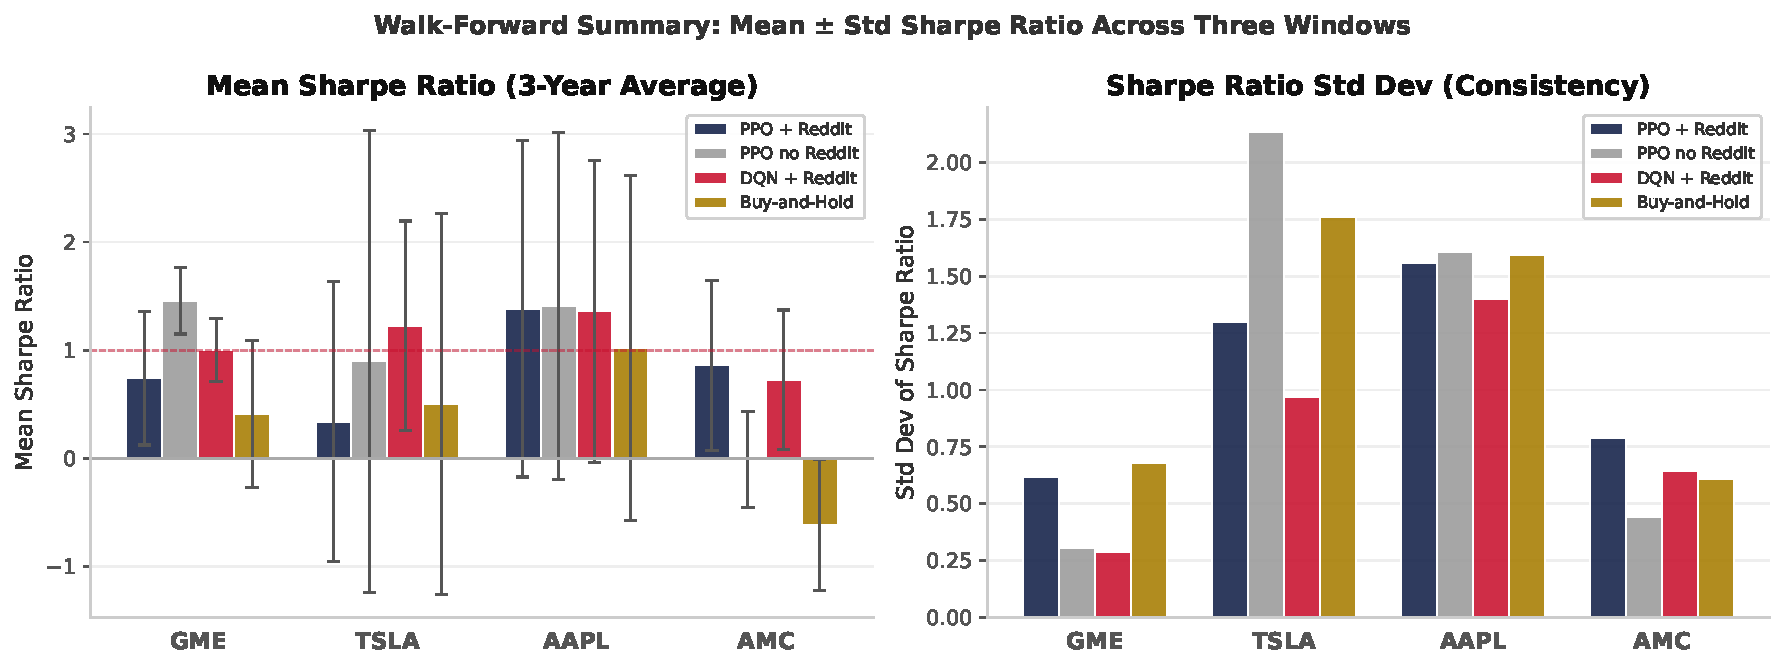
\includegraphics[width=\columnwidth]{walk_forward_summary.pdf}
  \caption{Mean Sharpe (left) and Sharpe std.\ dev.\ (right)
           across the three walk-forward windows.
           Error bars are $\pm 1$ standard deviation.
           DQN + Reddit is the most consistent agent on TSLA.
           PPO + Reddit dominates AMC.}
  \label{fig:wf_summary}
\end{figure}

\textbf{2022 (bear market).} Reddit matters a lot for AMC here.
This was the hardest year for equity markets in over a decade.
GME, TSLA, and AAPL all fell significantly.
The most dramatic result is AMC: PPO with Reddit returns
$+107.66\%$ while buy-and-hold loses $-83.07\%$.
This result deserves scrutiny because the action space
contains no shorting; the agent can only hold cash, buy all,
or sell all.
The gain came from timing AMC's August 2022 price spike.
AMC executed a 1-for-10 reverse stock split on August 22,
2022, and the surrounding corporate announcements (including
an ``APE'' preferred equity issuance) created extreme price
volatility: the split-adjusted price swung from roughly \$91
to \$254 within the same month.
The PPO agent with Reddit, reading the surge in community
activity around the corporate event, bought into the spike
and exited near the peak, producing more than 100\% return
from a small number of well-timed trades.
PPO without Reddit ($-64.98\%$) lacked this timing cue
and instead tracked AMC's broader downtrend throughout the
year, demonstrating that the Reddit embedding carried genuine
information about the timing of this event.
On TSLA, DQN with Reddit nearly breaks even ($-0.51\%$)
against a market that fell nearly 70\%, demonstrating that
the agent learned to exit before the worst of the drawdown.
GME is where things go wrong for Reddit: PPO with Reddit
achieves only Sharpe 0.052, while PPO without Reddit gets
1.778. This is discussed in detail below.

\textbf{2023 (recovery).} Reddit becomes noise in this window.
In a year when markets recovered and trended upward, the
Reddit signal lost most of its value.
On TSLA, PPO without Reddit achieves the highest result of
any model across all experiments: Sharpe 2.776 and
$+181.64\%$ return.
This makes sense: in a clear upward trend, an agent that just
follows price momentum will do very well.
Reddit discussion about TSLA tends to be contrarian or driven
by community drama around Musk that is unrelated to price;
in a strong uptrend the agent may read this negativity as a
sell signal when it is not one.
The results on AAPL are uniformly good (Sharpe above 2.3
for all models), consistent with the view that AAPL follows
macroeconomic trends rather than sentiment.

\textbf{2024 (mixed).} There is one notable failure in this window.
In 2024, PPO with Reddit achieves 137.54\% on GME, which is
the highest single-window result for that model.
This is because Roaring Kitty returned to social media in
May 2024 and GME spiked sharply; the Reddit embedding
captures this and the agent buys in.
However, PPO with Reddit fails completely on TSLA in 2024,
holding cash the entire year and returning 0\%, while the
no-Reddit PPO gets 89\% and buy-and-hold 67\%.
The TSLA community on Reddit in 2024 shifted significantly
as sentiment around Musk became more politically charged;
the embedding may have encoded this negativity as a sell
signal even as the stock performed well on fundamentals.

\textbf{The GME paradox.}
The most counterintuitive result in this paper is that Reddit
\emph{hurts} the PPO agent on GME across the walk-forward
windows (mean Sharpe 0.739 with Reddit vs 1.456 without).
GME is the stock most defined by Reddit, so this seems
backwards.

The explanation is a timing mismatch: the famous short squeeze
happened in January 2021, which falls in the training window
for all three walk-forward models.
The agent learns during training that high Reddit activity on
GME equals a price spike.
But in the test years (2022, 2023, 2024), that relationship
no longer holds.
The r/WallStreetBets community never stopped posting about
GME. There is an entire subculture of long-term GME holders
(``diamond hands'') who post enthusiastically regardless of
price.
In 2022 and 2023, Reddit posts about GME were frequent and
positive while the stock was declining.
The agent trained to associate positive GME Reddit activity
with price increases got the signal exactly backwards.
The no-Reddit agent, seeing only the declining price
momentum, correctly stayed in cash.

This is arguably the most important finding of the paper:
the Reddit signal for GME shifted from predictive (2021) to
misleading (2022--2023) as the community evolved.
A signal that worked historically can stop working precisely
because of how the community around it changes.

\subsection{When Does Reddit Help?}

Three patterns stand out across all experiments:

\textbf{Reddit helps when sentiment leads price.}
On TSLA and AMC, Reddit posts reflect evolving community views
(Musk news, declining interest in AMC) that sometimes precede
price movements.
The embedding encodes these shifts and the agent can act on
them.
The 2022 AMC result is the clearest example of this.

\textbf{Reddit does not help when price leads sentiment.}
In clear uptrends (TSLA 2023) or on institutionally-dominated
stocks (AAPL), price momentum is the more reliable signal.
The Reddit community often reacts to price moves rather than
causing them, so the embedding becomes a lagging indicator
that may mislead more than help.

\textbf{Reddit hurts when the community-price relationship
shifts.}
GME is the clearest example.
The correlation between Reddit activity and price moved from
positive (2021 squeeze) to uncorrelated or even negative
(2022--2023 holdout culture).
A model that learned the 2021 relationship and is tested in
2023 will systematically misread the signal.

% ─────────────────────────────────────────────────────────────
\section{Conclusion}

Whether Reddit improves a stock trading agent turns out to
depend heavily on which stock, which year, and whether the
community's relationship to the price is stable.

On TSLA, Reddit embeddings consistently improve both PPO and
DQN across most evaluation windows.
The signal seems to encode genuine information about
sentiment toward Musk's actions and TSLA news that leads
price.
On AMC, Reddit helps the agent recognise when retail interest
is collapsing and stay out of a declining stock, something
price features alone could not do as reliably.

On GME, the picture is more complicated.
The 80/20 split shows Reddit helping, largely because the
test period happens to include the 2024 Roaring Kitty spike.
But walk-forward validation over 2022--2023 shows Reddit
actively hurting the agent, because the community kept
posting bullishly about a stock that was falling.
The agent learned the wrong causal relationship from the 2021
training data and generalised it to a regime where it did not
apply.

Reddit is not uniformly helpful or harmful as a trading signal.
Its value depends on whether the community's sentiment is still
connected to actual price movements.
When it is, a Reddit-augmented agent can outperform by a
meaningful margin.
When that connection breaks down, the embedding becomes noise
or actively misleads the agent.
Future work should look at ways to detect when a community's
predictive power has decayed, and either down-weight or ignore
the embedding during those periods.
Online learning or periodically retraining the model with
recent data would also help the agent adapt to shifting
community dynamics rather than relying on patterns learned
years earlier.

\bibliographystyle{plainnat}
\bibliography{references}

\end{document}
